\begin{qBox}{5}
Produce several snapshots of the spin structure at \( 0.95 \times T_{ C } \).
Relate these observations to the correlation lengths you previously obtained.

\tcblower

Below are some snapshots of the spin structure at \( 0.95 \times T_{ C } \):
\begin{figure}[H]
    \centering
    \begin{minipage}{0.45\linewidth}
        \centering
        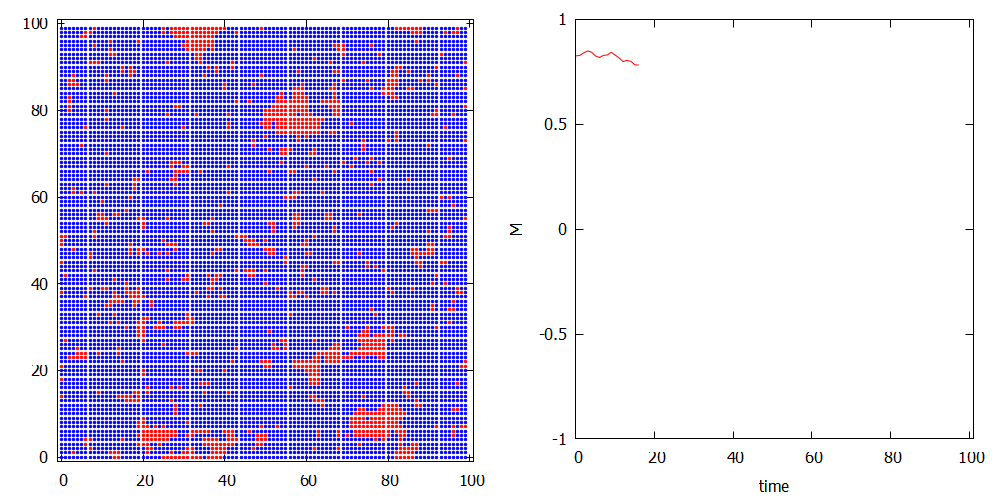
\includegraphics[ width = 0.95\linewidth ]{figures/sweep_16.png}
    \end{minipage}%
    \begin{minipage}{0.45\linewidth}
        \centering
        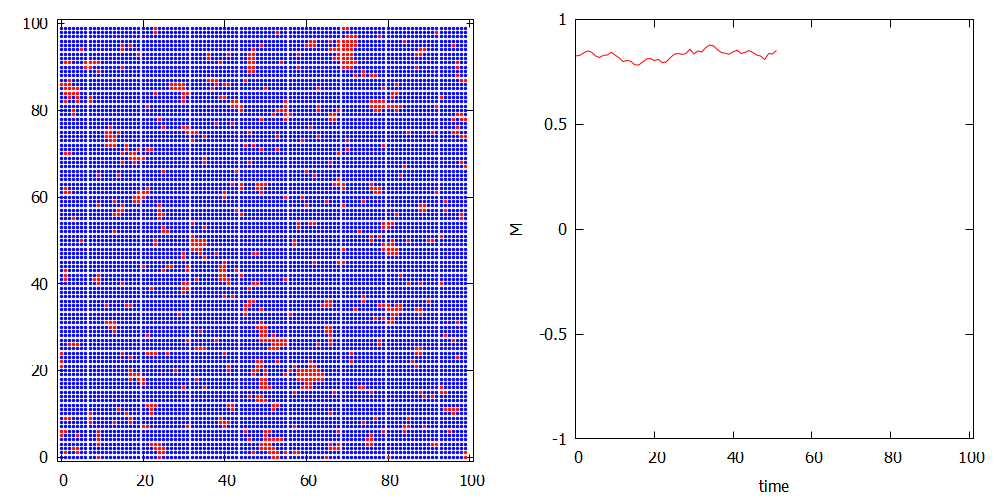
\includegraphics[ width = 0.95\linewidth ]{figures/sweep_51.png}
    \end{minipage}%
    \\
    \begin{minipage}{0.45\linewidth}
        \centering
        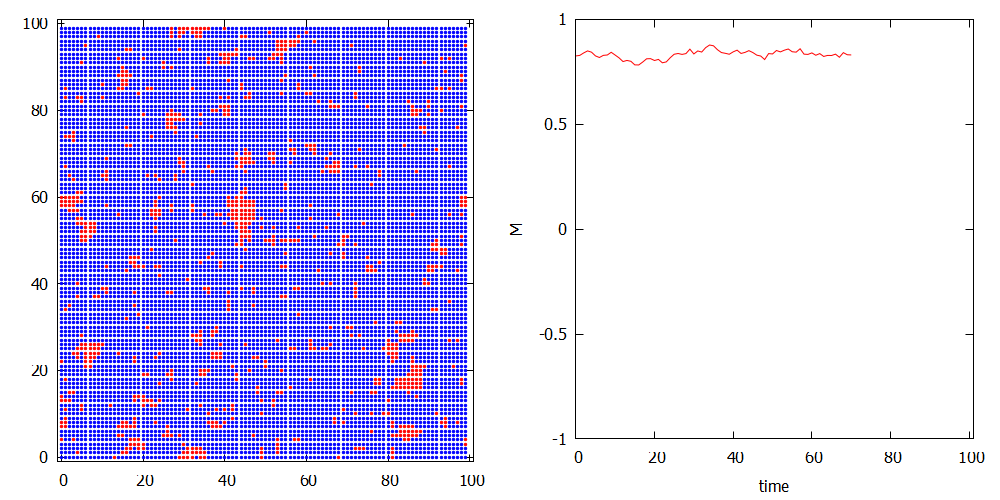
\includegraphics[ width = 0.95\linewidth ]{figures/sweep_70.png}
    \end{minipage}%
    \begin{minipage}{0.45\linewidth}
        \centering
        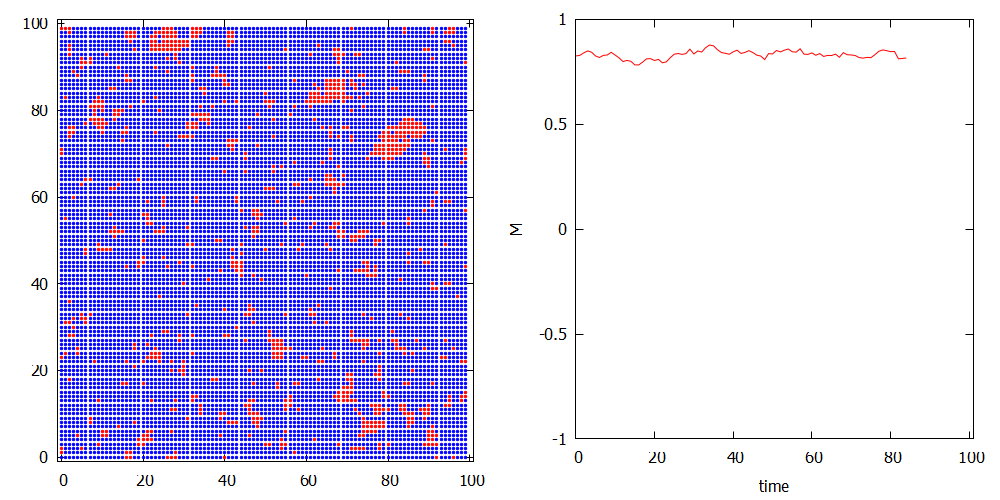
\includegraphics[ width = 0.95\linewidth ]{figures/sweep_84.png}
    \end{minipage}%
    \caption{Some snapshots of the spin structure at \( 0.95 \times T_{ C } \)}
\end{figure}
A gif can be found under the img folder.

\baseSkip 

From these snapshots, we see that there are clusters forming, which is a result of 
the spins being correlated to each other. 
Thus, the higher the correlation length we obtain, the larger we expect these 
clusters to be. 
Since \( 0.95 \times T_{ C } \) is near the critical temperature, we should expect 
clusters to form, which is indeed what we see. 

\baseSkip 

However, the correlation length that we found seems to be too small compared to the 
size of the clusters that are shown in the snapshots above; I think that we should 
instead expect a correlation length of around \( 10 \) based off the size of the 
clusters. 
The difference in the expected correlation length with the fitted correlation 
length is not a major concern for me since the fitted values have such a high 
uncertainty attached to them. 
If I were to refine the fitting some more (e.g., include weights to the data points, and maybe increase the number of sweeps), then I believe that we would see a more 
accurate value for the correlation length.
\end{qBox}